\documentclass[tikz,border=2pt]{standalone}
\usepackage{amsmath,amssymb}
\usepackage{tikz}
\usetikzlibrary{arrows.meta}

\begin{document}
% A Poisson number of arrivals (mean 20), each labelled urgent with probability 0.1 independently:
% the urgent and the ordinary counts are independent Poisson variables with means 2 and 18.
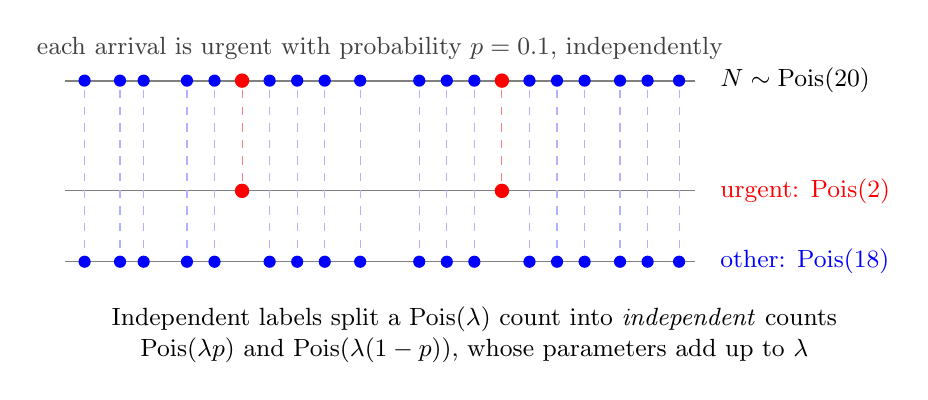
\begin{tikzpicture}[every node/.style={font=\small}, >={Latex[length=2mm]}]
	\draw[gray, thick] (0,0) -- (8,0);
	\draw[gray] (0,-1.4) -- (8,-1.4);
	\draw[gray] (0,-2.3) -- (8,-2.3);
	\foreach \x in {0.25, 0.7, 1.0, 1.55, 1.9, 2.6, 2.95, 3.3, 3.75, 4.5, 4.85, 5.2, 5.9, 6.25, 6.6, 7.05, 7.4, 7.8} {
		\fill[blue] (\x,0) circle (2.2pt);
		\fill[blue] (\x,-2.3) circle (2.2pt);
		\draw[blue!30, dashed] (\x,-0.12) -- (\x,-2.18);
	}
	\foreach \x in {2.25, 5.55} {
		\fill[red] (\x,0) circle (2.6pt);
		\fill[red] (\x,-1.4) circle (2.6pt);
		\draw[red!50, dashed] (\x,-0.12) -- (\x,-1.28);
	}
	\node[anchor=west] at (8.2,0) {$N\sim\operatorname{Pois}(20)$};
	\node[red, anchor=west] at (8.2,-1.4) {urgent: $\operatorname{Pois}(2)$};
	\node[blue, anchor=west] at (8.2,-2.3) {other: $\operatorname{Pois}(18)$};
	\node[anchor=south, font=\small, gray!50!black] at (4,0.15) {each arrival is urgent with probability $p=0.1$, independently};
	\node[anchor=north, align=flush center, text width=10.4cm] at (5.2,-2.75) {Independent labels split a $\operatorname{Pois}(\lambda)$ count into \emph{independent} counts $\operatorname{Pois}(\lambda p)$ and $\operatorname{Pois}(\lambda(1-p))$, whose parameters add up to $\lambda$};
\end{tikzpicture}
\end{document}
